\subsection{introduction}
	\begin{frame}\frametitle{fourier transform}\framesubtitle{introduction}
		\begin{figure}
			\centering
				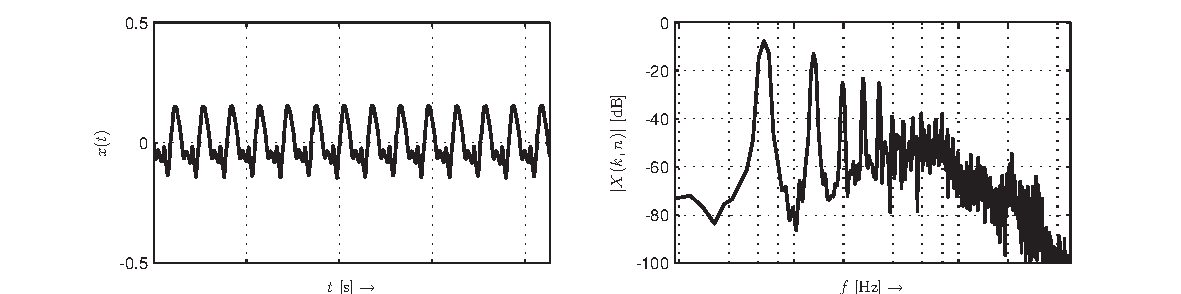
\includegraphics[scale=.5]{graph/fft}
		\end{figure}
		Fourier transform (structure):
		\begin{itemize}
			\item	continuous 
			\item	properties (continuous)
			\item	sampled time signals
			\item	short time (continuous)
			\pause
			\item	\textbf{DFT}
		\end{itemize}
	\end{frame}	
	\begin{frame}\frametitle{fourier transform}\framesubtitle{fourier series revisited}
			\begin {equation}
				c_k = \frac{1}{T_0}\int\limits_{-\nicefrac{T_0}{2}}^{\nicefrac{T_0}{2}} x(t) \e^{-\jom_0kt}\, dt \nonumber
			\end {equation}
        \only<1-4>{    
        \begin{itemize}
            \item   Fourier series coefficients can be interpreted as \textbf{correlation} ($\tau=0$) between signal and sinusoidals of different frequencies
            \item   only frequencies $k\omega_0$ are used
            ($\omega_0$ \textit{has to be known})
            \pause
            \item[$\Rightarrow$] Fourier series produces a \textbf{'line spectrum'}
            \bigskip
            \pause
            \item   distance between frequency components decreases as $T_0$ increases
            \pause
            \item[$\Rightarrow$]   aperiodic functions could be analyzed by increasing $T_0\rightarrow\infty$
        \end{itemize}
        }
        \only<5->{
        \begin{eqnarray*}
            &T_0 \rightarrow \infty&\\
            \pause
            \Rightarrow & k\omega_0 \rightarrow \omega\\
            \Rightarrow & \frac{1}{T_0} \rightarrow 0
        \end{eqnarray*}
        \pause
        \begin{itemize}
            \item[]   to avoid Zero result, multiply with $T_0$
        \end{itemize}
        }
        
        
        \vspace{70mm}
	\end{frame}	

\subsection{continuous Fourier transform}

	\begin{frame}\frametitle{fourier transform}\framesubtitle{definition (continuous)}
		\begin {equation*}\label{eq:fourier_transformation}
			X(\jom) = \mathfrak{F}[x(t)] = \int\limits_{-\infty}^{\infty} {x(t) \e^{-\jom t}\, dt}
		\end {equation*}
	\end{frame}	

	\begin{frame}\frametitle{fourier transform}\framesubtitle{example 1: rect window}
        \vspace{-8mm}
        \begin{footnotesize}
        \begin{eqnarray}
            w_{\mathrm{R}}(t)	&=& \left\lbrace  
                        \begin{array}{ll} 
                                                    1, & -\frac{1}{2} \leq t \leq \frac{1}{2}\\ 
                          \vphantom{\frac{1}{1}} 	0, & \text{otherwise} \\ 
                        \end{array} 
                        \right. .
        \end{eqnarray}
\pause
        \begin{eqnarray}
            W_{\mathrm{R}}(\jom) 	&=& \int\limits_{-\infty}^{\infty} {w_{\mathrm{R}}(t)\e^{-\jom t}\,dt}\nonumber\\
                        &=& \int\limits_{-\nicefrac{1}{2}}^{\nicefrac{1}{2}} {\e^{-\jom t}\,dt}\nonumber\\
                        &=& \frac{1}{-\jom} \underbrace{\left(\e^{-\mathrm{j}\nicefrac{\omega}{2}}-\e^{\mathrm{j}\nicefrac{\omega}{2}}\right)}_{= -2j\sin\left(\nicefrac{\omega}{2}\right)}\nonumber\\
                        &=& \frac{\sin\left(\nicefrac{\omega}{2}\right)}{\nicefrac{\omega}{2}} = \si\left(\frac{\omega}{2}\right) .
        \end{eqnarray}
        \end{footnotesize}
        \pause
        
        How will this change for different widths of $w_R$?
	\end{frame}	

	\begin{frame}\frametitle{fourier transform}\framesubtitle{example 2: dirac}
        \begin{eqnarray*} % is this a proper definition??????
            \int\limits_{-\infty}^{\infty} \delta(t)\, dt &=& 1\label{eq:dirac_int} ,\\
            \delta(t) &=& 0\; \text{for all } t\neq 0 .
        \end{eqnarray*}
        \pause
        \begin{equation*}
            \Rightarrow \Delta(\jom) = \int\limits_{-\infty}^\infty \delta(t)e^{-\jom t}dt = e^{-\jom \cdot 0} = 1
        \end{equation*}
        \pause
        
        \bigskip
        shifted dirac: $\delta(t-\tau_0)$
         \begin{equation*}
            \Rightarrow \Delta(\jom) = \int\limits_{-\infty}^\infty \delta(t-\tau_0)e^{-\jom t}dt = e^{-\jom \tau_0}
        \end{equation*}
   \end{frame}	

	\begin{frame}\frametitle{fourier transform}\framesubtitle{property 1: invertibility}
		\begin{eqnarray*}\label{eq:ift}
			x(t) &=& \mathfrak{F}^{-1}[X(\jom)]\nonumber\\
			 &=& \frac{1}{2\pi}\int\limits_{-\infty}^{\infty} X(\jom) \e^{\jom t}\, d\omega 
		\end{eqnarray*}
        \bigskip
 
        \begin{itemize}
            \begin{footnotesize}
            \item[] reminder: signal reconstruction with Fourier series coefficients
                \begin {equation*}
                    x(t) = \sum\limits_{k=-\infty}^{\infty} c_k e^{\jom_0kt}
                \end {equation*}
            \end{footnotesize}
            \pause
            \item   \textbf{comments}:
                \begin{itemize}
                    \item   invertibility: no information is lost during this process!
                    \item   FT and IFT are very similar, largely equivalent
                \end{itemize}
        \end{itemize}
        

	\end{frame}	

	\begin{frame}\frametitle{fourier transform}\framesubtitle{property 2: superposition}
		\begin{eqnarray}
			y(t) &=& c_1\cdot x_1(t) + c_2\cdot x_2(t)\nonumber\\
			\mapsto&&\nonumber\\
			Y(\jom) &=& c_1\cdot X_1(\jom) + c_2\cdot X_2(\jom)\nonumber
		\end{eqnarray}
		\pause
		\begin{itemize}
			\item[]	derivation
					\begin{footnotesize}
						\begin{eqnarray}
							Y(\jom) &=& \int\limits_{-\infty}^{\infty} {\big(c_1\cdot x_1(t) + c_2\cdot x_2(t)\big)\cdot \e^{-\jom t}\, dt}\nonumber\\
							\pause
							&=& c_1\cdot \int\limits_{-\infty}^{\infty} {x_1(t)  \e^{-\jom t}\, dt} + c_2\cdot \int\limits_{-\infty}^{\infty} {x_2(t) \e^{-\jom t}\, dt}\nonumber\\
							\pause
							&=& c_1\cdot X_1(\jom) + c_2\cdot X_2(\jom) 
						\end{eqnarray}
					\end{footnotesize}
		\end{itemize}
	\end{frame}	

	\begin{frame}\frametitle{fourier transform}\framesubtitle{property 3: convolution and multiplication}
		\vspace{-5mm}
        \begin{eqnarray}
			y(t) &= \int_{-\infty}^{\infty} {h(\tau) \cdot x(t-\tau)\, d\tau}\pause\mapsto 
			Y(\jom) &= H(\jom)\cdot X(\jom) \nonumber
		\end{eqnarray}
		\pause
		\begin{itemize}
			\item[]	derivation
					\begin{footnotesize}
				\begin{eqnarray}
					Y(\jom)	&=& \int_{-\infty}^{\infty} {y(t) \e^{-\jom t}\, dt}\nonumber\\
							\pause
								&=& \int_{-\infty}^{\infty} {\left(\int_{-\infty}^{\infty} {h(\tau) \cdot x(t-\tau)\, d\tau}\right) \e^{-\jom t}\, dt}\nonumber\\
							\pause
								&=& \int_{-\infty}^{\infty} {h(\tau) \int_{-\infty}^{\infty} {x(t-\tau)} \e^{-\jom t}\, dt\, d\tau}\nonumber\\
							\pause
								&=& \int_{-\infty}^{\infty} {h(\tau)  \e^{-\jom \tau} \underbrace{\int_{-\infty}^{\infty} {x(t-\tau)} \e^{-\jom (t-\tau)}\, d(t-\tau)}_{X(\jom)}\, d\tau}\nonumber\\
							\pause
								&=& \int_{-\infty}^{\infty} {h(\tau) \e^{-\jom \tau}\, d\tau} \cdot X(\jom)\nonumber\\
							\pause
								&=& H(\jom) \cdot X(\jom)\label{eq:mult_conv} 
				\end{eqnarray}
					\end{footnotesize}
		\end{itemize}
	\end{frame}	

	\begin{frame}\frametitle{fourier transform}\framesubtitle{property 4: Parseval's theorem}
		\begin{equation}
			\int_{-\infty}^{\infty}{x^2(t)\, dt} = \frac{1}{2\pi}\int_{-\infty}^{\infty} {\left|X(\jom)\right|^2\, d\omega} 
		\end{equation}
		\pause
		\begin{itemize}
			\item[]	derivation
			\begin{footnotesize}
				\begin{equation}
					\int_{-\infty}^{\infty}{h(\tau)\cdot x(t-\tau)\, d\tau} = \frac{1}{2\pi}\int_{-\infty}^{\infty} {H(\jom)\cdot X(\jom) \e^{\jom t} d\omega}\nonumber
				\end{equation}
				 \centering $H(\jom) \longrightarrow X^\ast (\jom)$/$h(\tau)\longrightarrow x(-\tau)$, $t = 0$
							\pause
				\begin{eqnarray}
					\int_{-\infty}^{\infty}{x(-\tau)\cdot x(-\tau)\, d\tau} &=& \frac{1}{2\pi}\int_{-\infty}^{\infty} {X^\ast (\jom)\cdot X(\jom) \, d\omega}\nonumber\\
					\pause
					\int_{-\infty}^{\infty}{x^2(t)\, dt} &=& \frac{1}{2\pi}\int_{-\infty}^{\infty} {\left|X(\jom)\right|^2\, d\omega} \nonumber
				\end{eqnarray}
			\end{footnotesize}
		\end{itemize}
	\end{frame}	

	\begin{frame}\frametitle{fourier transform}\framesubtitle{property 5: time \& frequency shift}
		\begin{equation}\label{eq:fft_timeshift}
			y(t) = x(t-t_0)\rightarrow Y(\jom) = X(\jom)\e^{-\jom t_0} 
		\end{equation} 
		\pause
		\begin{itemize}
			\item[]	derivation
			\begin{footnotesize}
				\begin{eqnarray}
					\int\limits_{-\infty}^{\infty} {x(t-t_0) \e^{-\jom t}\, dt} &=& \int\limits_{-\infty}^{\infty} {x(\tau) \e^{-\jom (\tau + t_0)}\, d\tau}\nonumber\\
					\pause
					&=& \e^{-\jom t_0}\int\limits_{-\infty}^{\infty} {x(\tau) \e^{-\jom \tau}\, d\tau}\nonumber\\
					\pause
					&=& \e^{-\jom t_0} \cdot X(\jom) \nonumber
				\end{eqnarray}
			\end{footnotesize}
		\end{itemize}
		\pause
		Frequency Shift:
		\begin{equation}
					\frac{1}{2\pi}\int\limits_{-\infty}^{\infty} X(\jom-\omega_0) \e^{\jom t}\, d\omega = \e^{\jom_0 t}\cdot x(t) 		
		\end{equation} 

	\end{frame}	

	\begin{frame}\frametitle[allowframebreaks]{fourier transform}\framesubtitle{property 6: symmetry 1/2}
		\begin{eqnarray}
			|X(\jom)| &=& |X(-\jom)|\\
			\Phi_\mathrm{X}(\omega) &=& -\Phi_\mathrm{X}(-\omega) 
		\end{eqnarray}
		\pause
		\vspace{-5mm}
		\begin{itemize}
			\item[]	derivation
			
			\begin{footnotesize}
				time signal sum of even and odd component $x_e(t), x_o(t)$:
				\begin{equation}
					x(t) = \underbrace{\frac{1}{2}(x(t) + x(-t))}_{x_e(t)} + \underbrace{\frac{1}{2}(x(t) - x(-t))}_{x_o(t)} 
				\end{equation}
				\pause
				\begin{equation}
					X_e(\jom) = \int\limits_{-\infty}^{\infty}{x_e(t)\cos(\omega t)\,dt} - \mathrm{j} \underbrace{\int\limits_{-\infty}^{\infty}{x_e(t)\sin(\omega t)\,dt}}_{= 0}\nonumber
				\end{equation}
				\pause
		\vspace{-5mm}
				\begin{itemize}
					\item[$\Rightarrow$]	$X_e(\jom)$ is real
					\item[$\Rightarrow$]	$X_e(\jom) = X_e(-\jom)$ (substitute $x(t)$ with $x(-t)$)
				\end{itemize}
			\end{footnotesize}
		\end{itemize}
	\end{frame}	

	\begin{frame}\frametitle[allowframebreaks]{fourier transform}\framesubtitle{property 6: symmetry 2/2}
		\begin{eqnarray}
			|X(\jom)| &=& |X(-\jom)|\\
			\Phi_\mathrm{X}(\omega) &=& -\Phi_\mathrm{X}(-\omega) 
		\end{eqnarray}
		\pause
		\vspace{-5mm}
		\begin{itemize}
			\item[]	derivation
			
			\begin{footnotesize}
				time signal sum of even and odd component $x_e(t), x_o(t)$:
				\begin{equation}
					x(t) = \underbrace{\frac{1}{2}(x(t) + x(-t))}_{x_e(t)} + \underbrace{\frac{1}{2}(x(t) - x(-t))}_{x_o(t)} 
				\end{equation}
				\pause
				\begin{equation}
					X_o(\jom) = \underbrace{\int\limits_{-\infty}^{\infty}{x_o(t)\cos(\omega t)\,dt}}_{=0} - \mathrm{j} \int\limits_{-\infty}^{\infty}{x_o(t)\sin(\omega t)\,dt} \nonumber
				\end{equation}
				\pause
		\vspace{-5mm}
				\begin{itemize}
					\item[$\Rightarrow$]	$X_o(\jom)$ is imaginary
					\item[$\Rightarrow$]	$X_o(\jom) = -X_o(-\jom)$ (substitute $x(t)$ with $-x(-t)$)
				\end{itemize}
			\end{footnotesize}
		\end{itemize}
	\end{frame}	

	\begin{frame}\frametitle{fourier transform}\framesubtitle{property 7: time \& frequency scaling}
				\begin{equation}
					y(t) = x(c\cdot t) \mapsto Y(\jom) = \frac{1}{|c|}X\left(j\frac{\omega}{c}\right) 
				\end{equation}
		\pause
		\begin{itemize}
			\item[]	derivation (positive c)
			\begin{footnotesize}
				\begin{eqnarray}
					Y(\jom) &=& \int\limits_{-\infty}^{\infty} {x(c\cdot t) \e^{-\jom t}\, dt}\nonumber\\
					\pause
					&=& \int\limits_{-\infty}^{\infty} {x(\tau) \e^{-\jom \frac{\tau}{c}}\, d\frac{\tau}{c}}\nonumber\\
					\pause
					&=& \frac{1}{c}\int\limits_{-\infty}^{\infty} {x(\tau) \e^{-\mathrm{j} \frac{\omega}{c} \tau}\, d\tau}\nonumber\\
					\pause
					&=& \frac{1}{c} X\left(\mathrm{j}\frac{\omega}{c}\right) \nonumber
				\end{eqnarray}
			\end{footnotesize}
		\end{itemize}
	\end{frame}	

	\begin{frame}\frametitle{fourier transform}\framesubtitle{examples}
			\begin{flushright}
				 
\includegraphics[scale=.08]{Graph/question-mark}
			\end{flushright}
			\vspace{-3mm}
			FT of:
			\begin{itemize}
				\item	delta function
				\item	constant
				\item	cosine
				\item	rectangular window
				\item	delta pulse
			\end{itemize}
	\end{frame}	

\subsection{Fourier transform of sampled signals}
	\begin{frame}\frametitle{fourier transform}\framesubtitle{sampled time signals 1/2}
		\vspace{-5mm}
        \begin{eqnarray}\label{eq:ft_sampled}
			\mathfrak{F}[x(i)] 	&=& \mathfrak{F}[x(t)\cdot \delta_\mathrm{T}(t)]\nonumber\\
			\pause
								&=& \mathfrak{F}[x(t)]\ast \mathfrak{F}[\delta_\mathrm{T}(t)]\nonumber\\
								&=& X(\jom)\ast \Delta_\mathrm{T}(\jom) \nonumber
		\end{eqnarray}
		\pause
        \visible<4->{
		transformed signal is 
        \begin{itemize}
            \item   still \textbf{continuous}
            \item   \textbf{periodic}
        \end{itemize}
        }
        \only<3>{
		\begin{figure}
			\centering
				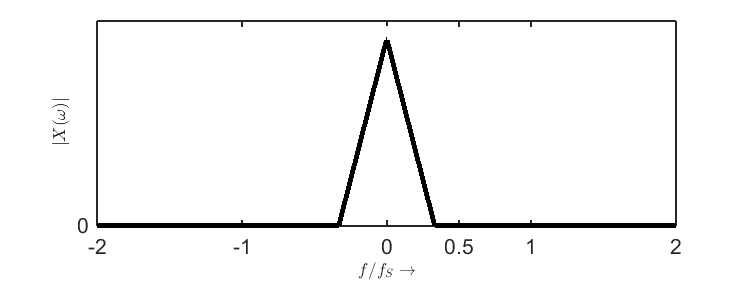
\includegraphics[scale=.7]{graph/spectrum_sampling_1}
		\end{figure}}
        \only<4>{
		\begin{figure}
			\centering
				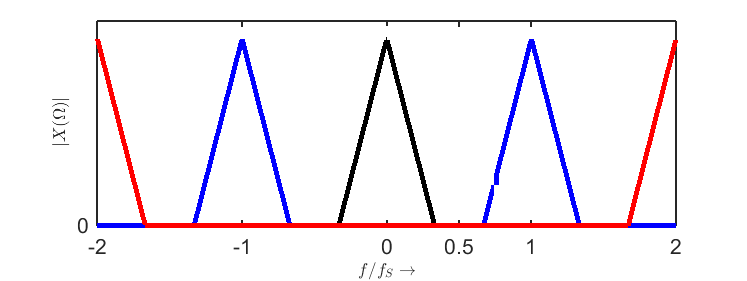
\includegraphics[scale=.7]{graph/spectrum_sampling_2}
		\end{figure}}
        \only<5->{
        \begin{center}
            \animategraphics[scale=.5,autoplay,loop]{10}{graph/SpectralAliasing/aliasing_}{1}{101}        
        \end{center}
        }
		%\begin{figure}
			%\centering
				%\includegraphics[scale=.7]{\AcaGraph/spectral_overlap}
		%\end{figure}
        \vspace{50mm}
	\end{frame}	
	\begin{frame}\frametitle{fourier transform}\framesubtitle{sampled time signals 2/2}
        \begin{eqnarray*}
            X(\jOm) &=& \sum\limits_{i=-\infty}^{\infty} x(i)e^{-\jOm i}\\
            x(i) &=& \frac{1}{2\pi}\int\limits_{-\pi}^{\pi}X(\jOm)e^{\jOm i} d\Omega\\
            \Omega &=& 2\pi\frac{\omega}{\omega_T}
        \end{eqnarray*}
	\end{frame}	

\subsection{Fourier transform of windowed signals}
	\begin{frame}\frametitle{fourier transform}\framesubtitle{STFT introduction}
		short time Fourier transform (STFT):\linebreak compute Fourier transform only over a segment

		\vspace{3mm}		
		\pause
		reasons:
		\begin{itemize}
			\item	\textbf{signal properties}: choose quasi-periodic segment
			\item	\textbf{perception}: ear analyzes short segments of signal
			\item	\textbf{hardware}: Fourier transform is inefficient and memory consuming for very long input segments
		\end{itemize}
		\pause
		$\Rightarrow$ multiply a \textbf{window} with the signal
	\end{frame}	

	\begin{frame}\frametitle{fourier transform}\framesubtitle{STFT: windowing}
        \begin{center}
            \animategraphics[scale=.8]{1}{graph/windowing/windowing_}{1}{5}        
        \end{center}
	\end{frame}	
    
	\begin{frame}\frametitle{fourier transform}\framesubtitle{STFT: spectrogram}
		\begin{figure}
			\centering
				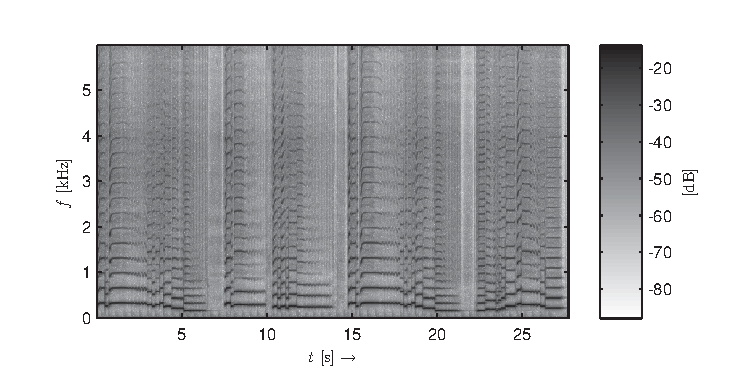
\includegraphics[scale=.85]{\AcaGraph/specgram}
		\end{figure}
	\end{frame}	

	\begin{frame}\frametitle{fourier transform}\framesubtitle{reminder: FT of rectangular window}
        \vspace{-8mm}
        \begin{footnotesize}
        \begin{eqnarray}
            w_{\mathrm{R}}(t)	&=& \left\lbrace  
                        \begin{array}{ll} 
                                                    1, & -L \leq t \leq L\\ 
                          \vphantom{\frac{1}{1}} 	0, & \text{otherwise} \\ 
                        \end{array} 
                        \right. .
        \end{eqnarray}
\pause
        \begin{eqnarray}
            W_{\mathrm{R}}(\jom) 	&=& \int\limits_{-\infty}^{\infty} {w_{\mathrm{R}}(t)\e^{-\jom t}\,dt}\nonumber\\
                        &=& \int\limits_{-L}^{L} {\e^{-\jom t}\,dt}\nonumber\\
                        &=& \frac{1}{-\jom} \underbrace{\left(\e^{-\mathrm{j}{\omega L}}-\e^{\mathrm{j}{\omega L}}\right)}_{= -2j\sin\left({L\omega}\right)}\nonumber\\
                        &=& \frac{2\sin\left({L\omega}\right)}{{\omega}}  .
        \end{eqnarray}
        \end{footnotesize}
        \pause
        Use the FT properties to derive the FT of a triangular window!
	\end{frame}	

	\begin{frame}\frametitle{fourier transform}\framesubtitle{STFT: window functions}
		multiplication in time domain $\rightarrow$ convolution in frequency domain
        \begin{equation*}
            x_\mathrm{W}(t) = x(t)\cdot w(t) \rightarrow X_\mathrm{W}(\jom) = X(\jom) \ast W(\jom)
        \end{equation*}

		\pause		
		$\Rightarrow$\textbf{spectral leakage}
		\begin{figure}
			\centering
				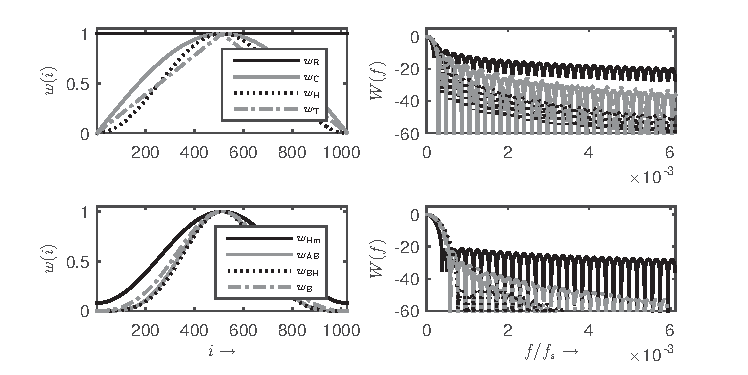
\includegraphics[scale=.8]{\AcaGraph/windows.pdf}
			\label{fig:windows}
		\end{figure}
	\end{frame}	

	\begin{frame}\frametitle{fourier transform}\framesubtitle{STFT: window function properties}
		\begin{itemize}
			\item	\textbf{main lobe width}
                \begin{itemize}
                    \item   how much does the main lobe ``smear'' a peak
                \end{itemize}
            \pause
			\item	\textbf{side lobe height}
                \begin{itemize}
                    \item   how dominant is the (highest) side lobe
                \end{itemize}
			\pause
            \item	\textbf{side lobe attenuation/fall-off}
                \begin{itemize}
                    \item   how much influence have distant sidelobes
                \end{itemize}
            \item   \textbf{process and scalloping loss} (DFT)
                \begin{itemize}
                    \item   how accurate is the amplitude (best case and worst case)
                \end{itemize}
		\end{itemize}
	\end{frame}	

	\begin{frame}\frametitle{fourier transform}\framesubtitle{STFT: typical window functions}
        \begin{itemize}
            \item   (rectangular window)
            \pause
            \smallskip
            \item   \textbf{von-Hann window}: $w_\mathrm{H}(t) = w_\mathrm{R}(t)\cdot\nicefrac{1}{2}\left(1 + \cos\left(\frac{\pi}{2}t\right) \right)$
            \pause
            \smallskip
            \item   \textbf{Hamming window}: $w_\mathrm{Hm}(t) = w_\mathrm{R}(t)\cdot\nicefrac{25}{46} + \nicefrac{42}{46}\cos\left(\frac{\pi}{2}t\right)$
            \pause
            \smallskip
            \item   \textbf{Cosine window}: $w_\mathrm{C}(t) = w_\mathrm{R}(t)\cdot\cos\left(\frac{\pi}{2}t\right)$
            \pause
            \smallskip
            \item   \textbf{Blackman-Harris window}:
                    \begin{equation}
						w_\mathrm{BH}(t) = w_{\mathrm{R}}(t)\sum\limits_{m=0}^{3}{b_m\cos\left(\frac{\pi}{2}mt\right)} .
					\end{equation}
                    with $b_0 = 0.35875,\, b_1 = 0.48829,\, b_2 = 0.14128, b_3 = 0.01168$
        \end{itemize}
	\end{frame}	


\subsection{discrete Fourier transform}
	\begin{frame}\frametitle{fourier transform}\framesubtitle{DFT}
		digital domain: requires discrete frequency values:
		
		$\Rightarrow$ \textbf{Discrete Fourier transform (DFT)}
		\begin{equation}
			X(k) = \sum\limits_{i=0}^{\mathcal{K}-1}{x(i)\e^{-\mathrm{j}ki\frac{2\pi}{\mathcal{K}}}}
		\end{equation}
        \pause
        alternative notation
		\begin{equation}
			X(k\Omega_\mathcal{K}) = \sum\limits_{i=0}^{\mathcal{K}-1}{x(i)\e^{-\mathrm{j}ki\Omega_\mathcal{K}}}
		\end{equation}
		
		\pause
        \bigskip
		2 interpretations:
		\begin{itemize}
			\item	sampled continuous Fourier transform
			\item	continuous Fourier transform of periodically extended time domain segment
		\end{itemize}
	\end{frame}	

	\begin{frame}\frametitle{fourier transform}\framesubtitle{DFT frequency resolution}
        \begin{itemize}
            \item   regular ``grid'' positions at $\omega = k\Omega_\mathcal{K} = k\frac{2\pi}{\mathcal{K}}$
            \pause
            \item   periodicity corresponds to sampling rate $\Rightarrow \Delta\omega = \frac{\omega_T}{\mathcal{K}}$
            \pause
            \item   increasing the DFT length increases frequency resolution
                \begin{itemize}
                    \item   decreasing time resolution
                    \item   zero-padding
                \end{itemize}
        \end{itemize}
	\end{frame}	
	\begin{frame}\frametitle{fourier transform}\framesubtitle{best case vs worst case}
		\begin{figure}
			\centering
				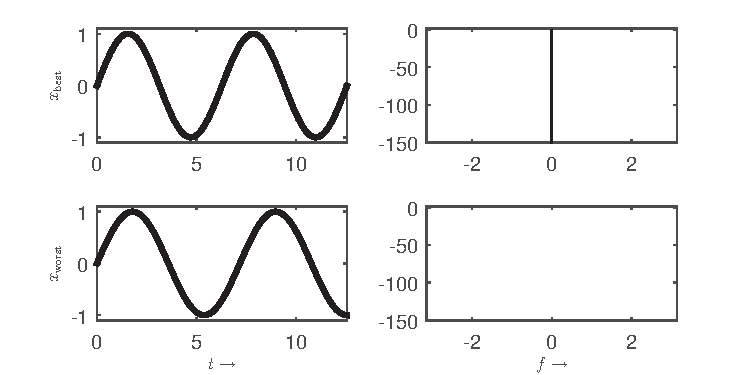
\includegraphics[scale=.7]{graph/bestworstcase}
		\end{figure}
	\end{frame}	

	\begin{frame}\frametitle{fourier transform}\framesubtitle{DFT vs FFT}
        \begin{itemize}
            \item   FFT is an algorithm to efficiently calculate the DFT
            \item   result is \textbf{identical}
            \item   efficiency:
                \begin{itemize}
                    \item   DFT: $\mathcal{K}^2$ complex multiplications
                    \item   FFT: $\nicefrac{\mathcal{K}}{2}\log_2(\mathcal{K})$ complex multiplications
                \end{itemize}
        \end{itemize}
        
        \begin{table}
            \centering
                \begin{tabular}{l|ccc}
                    $\mathcal{K}$  & DFT mult & FFT mult & efficiency\\ \hline
                    
                    $256$ & $2^{16}$ & $1024$ & $64:1$\\
                    $512$ & $2^{18}$ & $2304$ & $114:1$\\
                    $1024$ & $2^{20}$ & $5120$ & $205:1$\\
                    $2048$ & $2^{22}$ & $11264$ & $372:1$\\
                    $4096$ & $2^{24}$ & $24576$ & $683:1$\\
                \end{tabular}
        \end{table}
	\end{frame}	
    
\subsection{Fourier transform summary}
	\begin{frame}\frametitle{fourier transform}\framesubtitle{summary 1/2}
        \textbf{FT properties}
        \begin{enumerate}
            \item   invertibility
            \item   linearity
            \item   convolution --- multiplication
            \item   Parseval's theorem
            \item   time shift --- phase shift
            \item   symmetry
            \item   time scaling --- frequency scaling
        \end{enumerate}
	\end{frame}	
    
	\begin{frame}\frametitle{fourier transform}\framesubtitle{summary 2/2}
        \begin{enumerate}
            \item   Fourier series can describe any periodic function $\rightarrow$ discrete ``spectrum''
            \item   continuous FT transforms any continuous function $\rightarrow$ continuous spectrum
            \item   STFT transforms a segment of the signal $\rightarrow$ convolution with window spectrum
            \item   FT of sampled signals $\rightarrow$ periodic
            \item   DFT $\rightarrow$ sampled FT of periodic continuation
        \end{enumerate}
            \pause
        \begin{itemize}
            \item   \textbf{spectrum is periodic $\leftrightarrow$ time signal is discrete}
            \item   \textbf{spectrum is discrete $\leftrightarrow$ time signal is periodic}
        \end{itemize}
	\end{frame}	

%\begin{frame}{Fourier transform}{properties 1/4}
	%\begin{itemize}
		%\item	\textbf{invertibility}: the transformation is lossless
			%\begin{eqnarray}\label{eq:ift}
				%x(t) &=& \mathfrak{F}^{-1}\lbrace X(\jom)\rbrace \nonumber\\
				 %&=& \frac{1}{2\pi}\int\limits_{-\infty}^{\infty} X(\jom) \e^{\jom t}\enspace d\omega 
			%\end{eqnarray}
		%\pause
		%\item	\textbf{superposition}: the transformation is linear
		%\begin{eqnarray}
			%y(t) &=& c_1\cdot x_1(t) + c_2\cdot x_2(t)\nonumber\\
			%\mapsto&&\nonumber\\
			%Y(\jom) &=& c_1\cdot X_1(\jom) + c_2\cdot X_2(\jom)\nonumber
		%\end{eqnarray}
	%\end{itemize}
%\end{frame}	
%
%\begin{frame}{Fourier transform}{properties 2/4}
	%\begin{itemize}
		%\item	\textbf{convolution and multiplication}: replace each other in the other domain
		%\begin{eqnarray}
			%y(t) &= \int\limits_{-\infty}^{\infty} {h(\tau) \cdot x(t-\tau)\enspace d\tau}\mapsto 
			%Y(\jom) &= H(\jom)\cdot X(\jom) \nonumber
		%\end{eqnarray}
		%\pause
		%\item	\textbf{Parseval}: energy
		%\begin{equation}
			%\int\limits_{-\infty}^{\infty}{x^2(t)\enspace dt} = \frac{1}{2\pi}\int\limits_{-\infty}^{\infty} {\left|X(\jom)\right|^2\enspace d\omega} 
		%\end{equation}
	%\end{itemize}
%\end{frame}	
%
%\begin{frame}{Fourier transform}{properties 3/4}
	%\begin{itemize}
		%\item	\textbf{time shift}: scales phase spectrum
		%\begin{eqnarray}
			%y(t) &=& x(t-t_0)\mapsto \nonumber\\
			%Y(\jom) &=& X(\jom)\e^{-\jom t_0} 
		%\end{eqnarray}
		%\pause
		%\item	\textbf{frequency shift}: modulates time signal
		%\begin{equation}
			%\frac{1}{2\pi}\int\limits_{-\infty}^{\infty} X(\jom-\omega_0) \e^{\jom t}\enspace d\omega = \e^{\jom_0 t}\cdot x(t) 		
		%\end{equation}
	%\end{itemize}
%\end{frame}	
%
%\begin{frame}{Fourier transform}{properties 4/4}
	%\begin{itemize}
		%\item	\textbf{symmetry}: when $x(t)$ is real
		%\begin{eqnarray}
			%|X(\jom)| &=& |X(-\jom)|\\
			%\Phi_\mathrm{X}(\omega) &=& -\Phi_\mathrm{X}(-\omega) 
		%\end{eqnarray}
		%\pause
		%\item	\textbf{time/frequency scale}: inverse scaling relationship
			%\begin{eqnarray}
				%y(t) &=& x(c\cdot t) \mapsto\nonumber\\
				%Y(\jom) &=& \frac{1}{|c|}X\left(j\frac{\omega}{c}\right) 
			%\end{eqnarray}
	%\end{itemize}
%\end{frame}	
%
%\begin{frame}\frametitle{Fourier transform}\framesubtitle{examples}
	%\vspace{-15mm}
	%\begin{columns}
		%\column{5cm}
		%Describe the shape of the Fourier transform of the following signals:
		%
		%\column{4cm}
		%%\hspace{5mm}
		%\begin{flushright}
			 %
\includegraphics[scale=.08]{Graph/question-mark}
		%\end{flushright}
	%\end{columns}
%
	%\begin{itemize}
		%\item	delta function
		%\item	constant
		%\item	cosine
		%\item	rectangular window
		%\item	delta pulse
	%\end{itemize}
%\end{frame}	

